\chapter{Proceso de aprendizaje}
\label{cap:AnexoF}

Este anexo documenta la evolución del proceso de entrenamiento del clasificador CIE-10, desde los primeros experimentos exploratorios hasta la configuración final desplegada en producción.

Durante las fases de exploración (Fases~1--4), los experimentos se realizaron sobre la tarea de \textbf{clasificación de capítulos CIE-10} (21 clases) como aproximación de primer nivel: el menor número de clases permite ciclos de entrenamiento cortos y resultados interpretables, y el ranking relativo de modelos se transfiere bien a la tarea real. El \textbf{clasificador final de producción} opera sobre los 1.767 códigos CIE-10 completos (p.\,ej.\ \texttt{E11.9}) presentes en el conjunto de entrenamiento de CodiEsp.

\section{Fases de exploración}

El desarrollo del clasificador atravesó varias fases que se corresponden con los \emph{notebooks} del directorio \texttt{bert-classifier/}:

\subsection{Fase 0: análisis de la arquitectura jerárquica}

El \emph{notebook} \texttt{0\_\allowbreak{}clasificador\_\allowbreak{}jerarquico\_\allowbreak{}Introducción.ipynb} exploró la hipótesis de entrenar clasificadores independientes por nivel jerárquico (capítulo → bloque → código específico). Esta aproximación se descartó por la propagación de errores entre niveles, tal como se justifica en el ADR-05 (Anexo~\ref{cap:AnexoE}).

\subsection{Fase 1: RoBERTa-BSC base (evaluación)}

El \emph{notebook} \texttt{1\_\allowbreak{}clasificador\_\allowbreak{}jerarquico\_\allowbreak{}RoBERTa.ipynb} evaluó \texttt{PlanTL-GOB-ES/\allowbreak{}roberta-base-\allowbreak{}biomedical-clinical-es} como clasificador plano de primer nivel. El modelo se validó conceptualmente, pero no se llevó a producción: en el cribado de capítulos quedó a unos dos puntos de RigoBERTa-Clinical, dentro de la dispersión entre ejecuciones, y se prefirió el \emph{encoder} más próximo al dominio clínico y de mayor tamaño (véase el Anexo~\ref{cap:AnexoA}). La ventana de 512 tokens no distingue a ambos modelos, porque RigoBERTa-Clinical tiene la misma.

\subsection{Fase 2: IIC/RigoBERTa-2.0 (evaluación)}

El \emph{notebook} \texttt{2\_\allowbreak{}clasificador\_\allowbreak{}jerarquico\_\allowbreak{}RigoBERTa.ipynb} introdujo \texttt{IIC/RigoBERTa-2.0}~\cite{vacaserrano2022rigoberta}, versión de propósito general de RigoBERTa sobre arquitectura XLM-RoBERTa-large. Este modelo se evaluó conceptualmente como punto de partida previo a la variante clínica.

\subsection{Fase 3: mmBERT (primeros entrenamientos experimentales)}

El \emph{notebook} \texttt{5\_\allowbreak{}clasificador\_\allowbreak{}jerarquico\_\allowbreak{}mmBert.ipynb} inició los experimentos con entrenamiento real sobre el corpus CodiEsp~\cite{miranda2020}. Se realizaron 8 ejecuciones con \texttt{jhu-clsp/mmBERT-base} sobre 809 códigos de bloque, con F1-micro entre 0{,}03 y 0{,}15.

\subsection{Fase 4: ModernBERT (evaluación)}

El \emph{notebook} \texttt{4\_\allowbreak{}clasificador\_\allowbreak{}jerarquico\_\allowbreak{}ModernBert.ipynb} evaluó la arquitectura ModernBERT~\cite{warner2024modernbert}, que obtuvo un F1-micro de 0{,}632 en pruebas de nivel~1 con el mismo presupuesto que los demás candidatos. No se llevó más allá porque está entrenado únicamente en inglés; queda identificado como candidato para iteraciones futuras (véase el Anexo~\ref{cap:AnexoA}).

\subsection{Fase 5: IIC/RigoBERTa-Clinical (entrenamiento intensivo)}

A partir de la ejecución 9 se adoptó \texttt{IIC/RigoBERTa-Clinical}~\cite{garciasubies2026rigobertaclinical} como modelo base. La fase 5 comprende 53 ejecuciones (de la 9 a la 62, excluida la 20, dedicada al Longformer-BSC) en las que se ajustaron progresivamente los hiperparámetros: tasa de aprendizaje, congelación de capas, descongelación progresiva, \emph{dropout}, \emph{pos\_weight\_cap}, \emph{label smoothing} y umbral de clasificación. El F1-micro de validación pasó de 0{,}32 (primera ejecución) a 0{,}4945 (ejecución 55, la mejor de las 62 y modelo de referencia hasta la promoción de \texttt{zlpr-map}, Anexo~\ref{cap:AnexoH}).

\subsection{Fase 6: análisis de nivel 2}

El \emph{notebook} \texttt{7\_\allowbreak{}clasificador\_\allowbreak{}jerarquico\_\allowbreak{}analisis\_nivel\_2.ipynb} analizó la viabilidad de extender el clasificador plano a 4 caracteres (nivel de bloque específico). Se concluyó que las frecuencias de entrenamiento por código son insuficientes en el corpus actual para este nivel de especificidad.

\section{Evolución de los entrenamientos}

La Tabla~\ref{tab:training-evolution} recoge los hitos más relevantes de las 62 ejecuciones de esta fase de optimización del F1-micro: 8 con mmBERT, 1 de comparación con Longformer-BSC (descartado por coste computacional, véase el Anexo~\ref{cap:AnexoA}) y 53 con RigoBERTa-Clinical. A ellas se suman dieciséis ejecuciones dirigidas al MAP: las seis de la sección~\ref{sec:anexoF-map} (control, ajuste, ampliación del promedio y destilación) y las diez de las secciones siguientes (tres del paso~40, tres de continuación, dos semillas adicionales y dos réplicas de control). El registro completo suma 78 ejecuciones.

\begin{table}[H]
\centering
\caption{Hitos representativos del proceso de entrenamiento. Elaborada a mano a partir de las filas homónimas de \texttt{ai\_engine/\allowbreak model/\allowbreak training\_runs.csv} (el número de ejecución es el de la fila); no tiene objetivo de \texttt{make}. La serie completa se dibuja con \texttt{make ai-tfg-figures} (Figura~\ref{fig:all-trainings}).}
\label{tab:training-evolution}
\begin{tabular}{clcrcP{4.0cm}}
\hline
\textbf{Ejec.} & \textbf{Modelo} & \textbf{Códigos} & \textbf{Épocas} & \textbf{F1-micro} & \textbf{Observación} \\
\hline
1 & mmBERT & 809 & 19 & 0{,}061 & Línea base inicial \\
8 & mmBERT & 809 & 20 & 0{,}150 & Mejor mmBERT \\
9 & RigoBERTa-Clinical & 809 & 20 & 0{,}320 & Cambio de modelo (+113\% sobre mmBERT) \\
18 & RigoBERTa-Clinical & 809 & 133 & 0{,}430 & Mejor con 809 códigos \\
21 & RigoBERTa-Clinical & 1.767 & 79 & 0{,}327 & Expansión a espacio completo \\
27 & RigoBERTa-Clinical & 1.767 & 60 & 0{,}470 & Introducción descongelación prog. \\
39 & RigoBERTa-Clinical & 1.767 & 96 & 0{,}481 & Ajuste umbral y \emph{pos-weight} \\
44 & RigoBERTa-Clinical & 1.767 & 150 & 0{,}489 & Configuración 32b de referencia \\
55 & RigoBERTa-Clinical & 1.767 & 150 & 0{,}4945 & Referencia de evaluación (paso 36) \\
67 & RigoBERTa-Clinical & 1.767 & 112 & 0{,}5028 & Mejor ejecución registrada hasta la fecha \\
\hline
\end{tabular}
\end{table}

\section{Comparativa de ejecuciones}

La Figura~\ref{fig:all-trainings} muestra el F1-micro de validación de cada ejecución registrada, en orden cronológico, y las épocas que ejecutó cada una.

\begin{figure}[!ht]
\centering
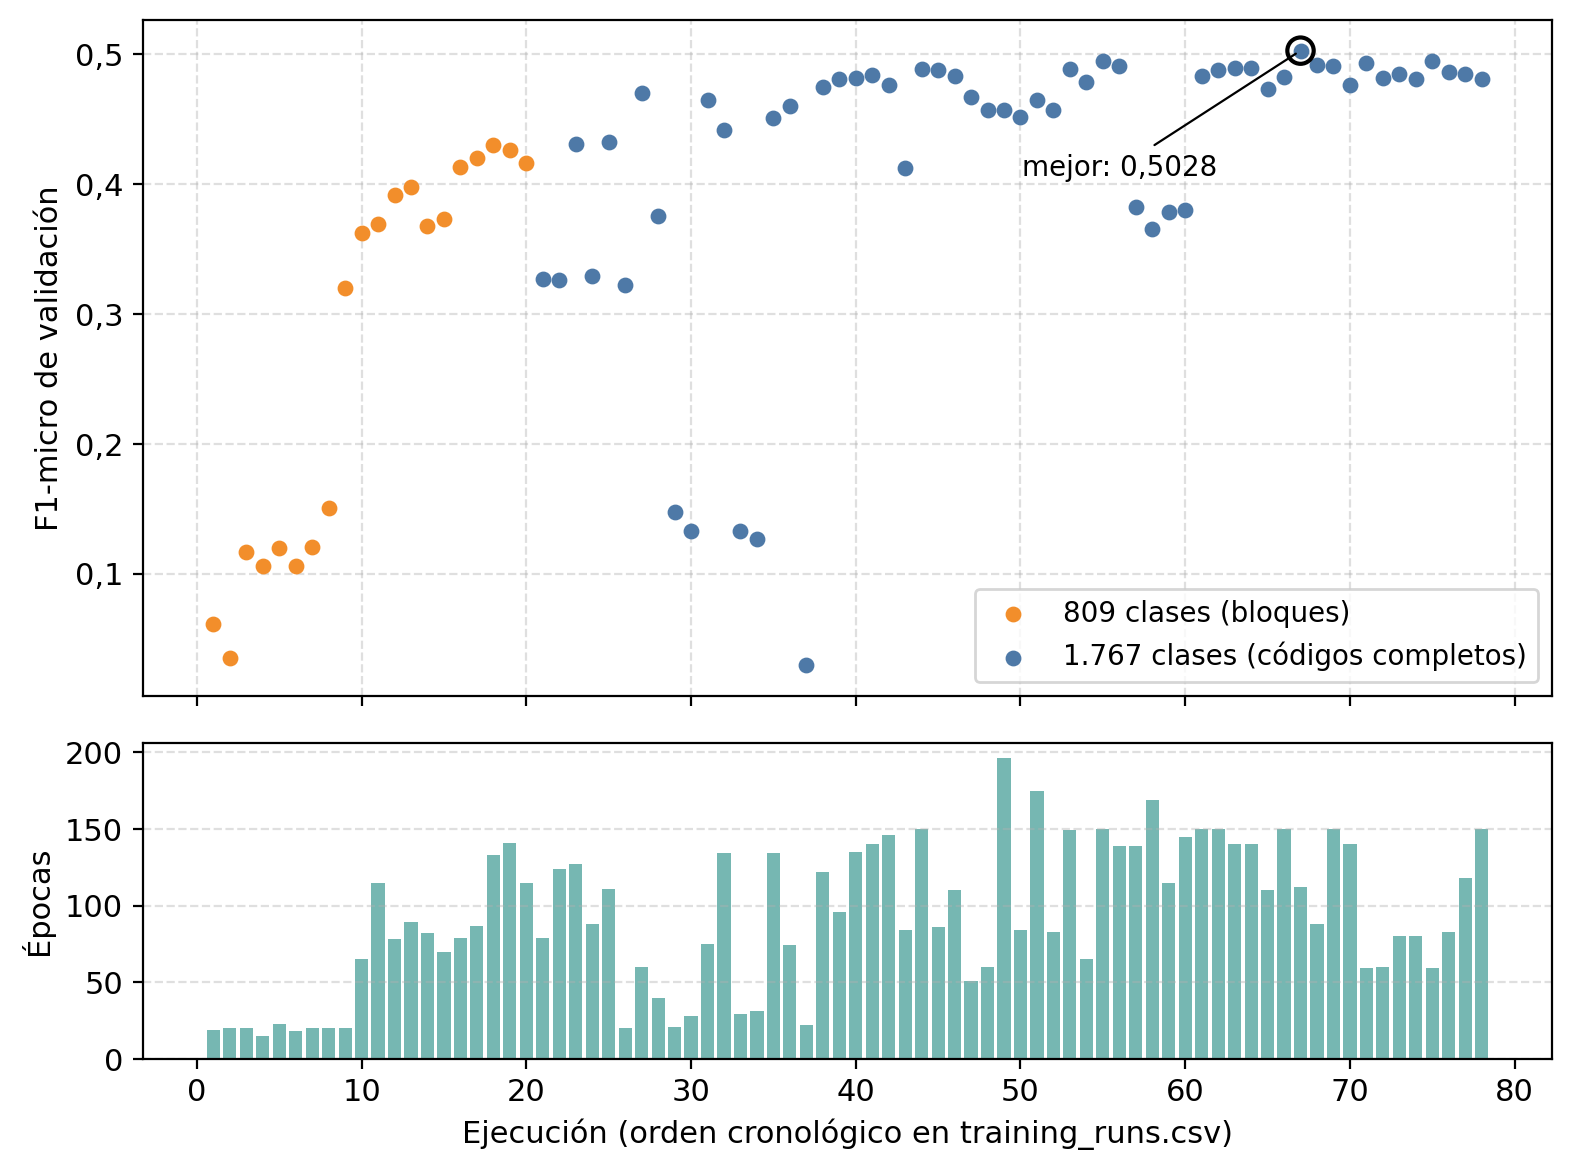
\includegraphics[width=\textwidth]{figs/all_trainings_graph}
\caption{F1-micro de validación (arriba) y épocas ejecutadas (abajo) de cada ejecución, en orden cronológico. Azul: 1.767 clases; naranja: 809 clases. El círculo marca la mejor ejecución con 1.767 clases. Generada con \texttt{make ai-tfg-figures} (\texttt{ai\_engine/plot\_runs.py}) a partir de \texttt{model/training\_runs.csv}.}
\label{fig:all-trainings}
\end{figure}

\section{Optimización específica del MAP}
\label{sec:anexoF-map}

Las 62~ejecuciones anteriores optimizaron el F1-micro, por las razones expuestas en el capítulo de desarrollo. El MAP por documento, sin embargo, es la métrica oficial del \emph{benchmark} CodiEsp y la única homogénea con los sistemas participantes, por lo que se realizó una serie de experimentos dirigidos específicamente a mejorarla.

\paragraph{Procedencia de las cifras de esta sección.}
El mismo modelo aparece con dos valores según la pasada de evaluación. Las cifras del modelo del paso~36 (MAP de prueba 0,4373; F1-micro 0,4887) proceden de \texttt{eval\_test.py} en precisión completa y fueron las cifras titulares hasta que la comparación de candidatos en prueba (Anexo~\ref{cap:AnexoH}, sección~\ref{sec:anexoH-candidatos}) promocionó \texttt{zlpr-map}; el cuerpo de la memoria cita ahora 0,454 y 0,495 para ese modelo. Las tablas de esta sección son anteriores a esa promoción y \textbf{comparan varias ejecuciones entre sí} con \texttt{ensemble\_eval.py}, en precisión reducida, donde el modelo del paso~36 da 0,4342 en prueba y 0,4343 en validación (\texttt{eval\_paso40.json}). Cada tabla indica sus ficheros de origen, todos ellos salidas de ese guion, y usa esa fila para el paso~36. Las pasadas difieren entre sí en la tercera o cuarta cifra decimal (por ejemplo, 37a da 0,4389 en \texttt{ensemble\_eval.json} y 0,4390 en \texttt{ensemble\_eval5.json}; la ejecución 41b da 0,4533 y 0,4535 en dos pasadas). Esas diferencias no alteran ninguna conclusión, pero mezclar ambas procedencias al citar produciría una contradicción aparente. Salvo indicación expresa, el MAP de las tablas es el de prueba sobre el \emph{gold} completo; los diferenciales derivados se calculan dentro de una misma procedencia.

\subsection{Variabilidad estocástica como referencia}

Antes de atribuir una mejora a cualquier cambio es necesario conocer el ruido del proceso. Dos ejecuciones con configuración \textbf{idéntica} (\texttt{20260530T030233Z} y \texttt{20260530T134649Z}) obtuvieron MAP de 0{,}5442 y 0{,}5317 en validación: una dispersión de \textbf{1{,}25~puntos porcentuales} atribuible únicamente a la inicialización aleatoria y al no determinismo del entrenamiento en GPU. Esa cifra está medida sobre el MAP de validación restringido al vocabulario del modelo, que es la métrica que registraba el entrenamiento en ese momento, y sobre dos ejecuciones. La subsección~\ref{sec:anexoF-distribuciones} la sustituye por una estimación con cinco réplicas sobre la métrica que de verdad decide, el MAP del \emph{gold} completo en prueba: desviación típica de 0{,}0051 y rango de 1{,}06~pp. Con cualquiera de las dos lecturas la conclusión operativa es la misma: una diferencia inferior al punto porcentual no puede atribuirse con seguridad a un cambio a partir de una sola ejecución.

\subsection{Selección de checkpoint por MAP}

Hasta este punto, el mejor \emph{checkpoint} y el planificador de la tasa de aprendizaje (\emph{scheduler}) \texttt{ReduceLROnPlateau} se gobernaban por el F1-micro de validación. Se incorporó el parámetro \texttt{--select\_metric} para poder guiarlos por el MAP, y se registró además el MAP de cada época en el historial de entrenamiento, que hasta entonces no se almacenaba.

El análisis del historial de la ejecución de control mostró que el margen disponible era pequeño: el MAP máximo (0{,}5501, época~88) apenas superaba en 0{,}24~pp al MAP de la época elegida por F1 (0{,}5477, época~103), y permanecía prácticamente plano entre las épocas~70 y~124. La ejecución completa (Tabla~\ref{tab:map-experiments}) apunta a que el cambio es contraproducente: guiar el planificador por una métrica plana parece degradar la trayectoria de aprendizaje completa.

\subsection{Calibración entre clases}

El MAP evalúa el \emph{ranking} de códigos dentro de cada documento, de modo que el \texttt{pos\_weight} por clase (que desplaza los \emph{logits} de cada código en distinta magnitud) podría estar distorsionando esa comparación. Se redujo \texttt{pos\_weight\_cap} de 10 a 3, con resultado también negativo tanto en MAP como en F1. La Tabla~\ref{tab:map-experiments} recoge ambos experimentos junto con la ejecución de control.

\begin{table}[h]
\centering
\caption{Experimentos dirigidos a mejorar el MAP. Todos parten de la configuración de producción (paso~36). MAP de validación restringido al vocabulario del modelo y F1-micro de validación, de \texttt{model/\allowbreak ensemble\_eval.json}. Generada con \texttt{python3 ensemble\_eval.py --ckpts} \emph{checkpoints} \texttt{--labels} etiquetas (sin objetivo de \texttt{make}); la salida es ese JSON.}
\label{tab:map-experiments}
\begin{tabular}{lP{6.0cm}cc}
\hline
\textbf{Ejec.} & \textbf{Cambio respecto a producción} & \textbf{MAP val} & \textbf{F1-micro val} \\
\hline
37ctrl & Ninguno (control, otra semilla) & 0{,}5477 & 0{,}4884 \\
37a & \texttt{select\_metric=map\_macro} & 0{,}5365 & 0{,}4902 \\
37b & \texttt{select\_metric=map\_macro} + \texttt{pos\_weight\_cap=3} & 0{,}5202 & 0{,}4743 \\
\hline
\end{tabular}
\end{table}

\subsection{Observación incidental: promediado de las ejecuciones}

Una variabilidad de 1{,}25~pp sugiere que reducir la varianza puede ser más rentable que perseguir configuraciones marginalmente mejores. Para comprobarlo se promediaron las probabilidades de salida de los tres \emph{checkpoints} anteriores, con los resultados de la Tabla~\ref{tab:map-ensemble}. Esta prueba tiene un alcance limitado: los tres \emph{checkpoints} no se entrenaron para combinarse, sino que persiguen objetivos distintos (un control y dos variantes que, individualmente, resultaron peores). No se trata, por tanto, de un sistema de combinación diseñado ni evaluado como tal, sino de una comprobación posterior sobre los modelos disponibles. Por ese motivo el resultado no se reporta como resultado de este trabajo ni se emplea en la comparación con el \emph{benchmark}, que utiliza el modelo de producción.

\begin{table}[h]
\centering
\caption{MAP por documento sobre el conjunto de prueba: modelos individuales frente a su promedio. El promedio no constituye un sistema propuesto (véase el texto). Las filas 37a y promedio proceden de \texttt{model/\allowbreak ensemble\_eval.json}; la fila del paso~36, de \texttt{model/\allowbreak eval\_paso40.json} (mismo guion, otra pasada). Generada con \texttt{python3 ensemble\_eval.py} (sin objetivo de \texttt{make}).}
\label{tab:map-ensemble}
\begin{tabular}{lcc}
\hline
\textbf{Modelo} & \textbf{MAP (gold completo)} & \textbf{MAP (vocabulario)} \\
\hline
Producción (paso~36) & 0{,}4342 & 0{,}5326 \\
Mejor individual (37a) & 0{,}4389 & 0{,}5393 \\
Promedio de los 3 & 0{,}4683 & 0{,}5728 \\
\hline
\end{tabular}
\end{table}

El promedio supera al modelo de producción en 3{,}41~pp de MAP sobre el gold completo y al mejor modelo individual en 2{,}9~pp, más de dos veces la dispersión entre semillas (1,06~pp de rango, Tabla~\ref{tab:map-distribuciones}), y el efecto se reproduce en validación. El coste sería triplicar el tiempo de inferencia y el espacio de almacenamiento, incompatible con el requisito de latencia del sistema. La conclusión que cabe extraer es metodológica: existe margen de mejora por esta vía, y diseñar y evaluar una combinación de modelos de forma rigurosa queda planteado como trabajo futuro.

\subsection{Destilación del promedio}

El promediado deja una pregunta abierta: si la ganancia existe pero no cabe en el presupuesto de inferencia, ¿puede transferirse a un único modelo? La vía estándar es la destilación de conocimiento~\cite{hinton2015distilling}: entrenar un clasificador nuevo (alumno) contra las probabilidades que produce el promedio (profesor), en lugar de contra las etiquetas binarias del corpus. La hipótesis es que las probabilidades del profesor contienen información que las etiquetas no tienen (sobre todo en los negativos, donde el orden relativo entre códigos plausibles y códigos absurdos es precisamente lo que mide el MAP) y que el alumno puede aprenderla conservando el coste de inferencia de un solo modelo.

Se amplió primero el promedio de tres a cinco ejecuciones (Tabla~\ref{tab:map-distill}) y se entrenó el alumno con una pérdida mixta $\alpha \cdot \mathcal{L}_{\text{blanda}} + (1-\alpha) \cdot \mathcal{L}_{\text{dura}}$ con $\alpha = 0{,}5$, siendo $\mathcal{L}_{\text{blanda}}$ la entropía cruzada binaria contra las probabilidades del profesor.

\begin{table}[h]
\centering
\caption{Destilación del promedio de cinco ejecuciones. MAP por documento sobre el gold completo. Rango y promedio de \texttt{model/\allowbreak ensemble\_eval5.json}, alumno de \texttt{model/\allowbreak eval\_distill.json} y paso~36 de \texttt{model/\allowbreak eval\_paso40.json}. Generada con \texttt{python3 ensemble\_eval.py} (sin objetivo de \texttt{make}).}
\label{tab:map-distill}
\begin{tabular}{P{6.0cm}cc}
\hline
\textbf{Modelo} & \textbf{MAP validación} & \textbf{MAP prueba} \\
\hline
Producción (paso~36) & 0{,}4343 & 0{,}4342 \\
Cinco ejecuciones previas disponibles (rango)$^{*}$ & 0{,}4166--0{,}4442 & 0{,}4192--0{,}4421 \\
Promedio de las cinco & 0{,}4715 & 0{,}4778 \\
Alumno destilado & 0{,}4299 & 0{,}4354 \\
\hline
\end{tabular}

\vspace{2mm}
{\footnotesize $^{*}$ Dos de esas cinco ejecuciones no eran réplicas de la configuración de producción sino variantes descartadas, lo que rebajaba la media del grupo. La subsección~\ref{sec:anexoF-distribuciones} documenta el error y rehace la comparación con el grupo corregido.}
\end{table}

El alumno no recupera ganancia apreciable: su MAP de prueba queda dentro del rango de las ejecuciones individuales y 4{,}2~pp por debajo del profesor. El diagnóstico está en las probabilidades del profesor sobre el conjunto de entrenamiento, que es donde el alumno aprende: la probabilidad media asignada a los códigos positivos es del 97~\% y el 99{,}5~\% de ellos supera el 0{,}9. Con 500 documentos y 150~épocas, los profesores prácticamente memorizan el corpus de entrenamiento, de modo que sus probabilidades se reducen a las etiquetas binarias y la pérdida blanda no aporta señal adicional. La estructura fina de los negativos, que era la apuesta del experimento, tampoco basta: con $\alpha=0{,}5$ y probabilidades negativas del orden de $10^{-3}$, ese término queda aplastado por la contribución de los positivos.

La lección no es que la destilación no funcione, sino que no funciona \emph{en este régimen}: exige un profesor que generalice sobre los datos que ve el alumno, y con 500 documentos el profesor no generaliza sobre ellos, los memoriza. Destilar sobre un corpus no etiquetado y disjunto del de entrenamiento (donde el profesor sí produciría probabilidades informativas) es la variante que quedaría por probar, y requiere textos clínicos adicionales de los que este trabajo no dispone.

\subsection{Alinear la pérdida con la métrica}
\label{sec:anexoF-alineacion}

Los experimentos anteriores comparten un supuesto que conviene revisar: todos ajustan el proceso de entrenamiento (qué \emph{checkpoint} se elige, cómo se pondera cada clase, con qué semilla se arranca) manteniendo intacta la función de pérdida. Y esa función es una entropía cruzada binaria que trata cada uno de los 1.767 códigos como un problema independiente: optimiza que la probabilidad de cada código esté bien calibrada por separado. El MAP mide algo distinto, que los códigos correctos de un informe queden por encima de los incorrectos \emph{de ese mismo informe}. Un ajuste de hiperparámetros difícilmente puede corregir esa desalineación, porque el objetivo que se minimiza sigue siendo otro. A esto se suma el diagnóstico acumulado en las secciones anteriores: el ruido entre semillas idénticas (en torno a 1~pp sobre el conjunto de prueba, según la estimación con réplicas de la subsección~\ref{sec:anexoF-distribuciones}) es del orden del efecto de cualquier cambio de hiperparámetro ensayado, y lo que más ha movido el MAP hasta ahora (promediar varias ejecuciones, $+4{,}36$~pp sobre el paso~36 con cinco ejecuciones) es inviable en producción por coste de inferencia.

De ahí salen tres ejecuciones, cada una atacando uno de esos tres diagnósticos. Todas parten de la configuración de producción y modifican un solo elemento, de forma que sus efectos sean atribuibles por separado, y ninguna altera el coste de inferencia: los tres cambios viven exclusivamente en el entrenamiento.

\subsubsection*{Ejecución 40a: pérdida listwise por documento (ZLPR)}

\textbf{Diagnóstico que ataca.} La desalineación entre pérdida y métrica.

\textbf{Mecanismo.} Se añade a la entropía cruzada el término~\cite{su2022zlpr}
\[
\mathcal{L}_{\text{ZLPR}} = \log\Big(1 + \sum_{j \in \text{neg}} e^{z_j}\Big) + \log\Big(1 + \sum_{i \in \text{pos}} e^{-z_i}\Big),
\]
mínimo cuando todos los códigos correctos de un documento superan a todos los incorrectos del mismo documento, sin exigir ningún valor absoluto concreto a ninguno. Es la traducción directa del MAP a una función derivable. El peso, 0{,}1, se fijó midiendo ambos términos en una ejecución de prueba de una época: con ese factor la entropía cruzada aporta 0{,}74 y el término de ordenación 1{,}02, escalas comparables.

\textbf{Qué se espera.} Es la que actúa sobre la causa y no sobre un síntoma, así que es la candidata con mayor recorrido: una mejora de 2~a~4~pp de MAP la situaría por encima del ruido. El riesgo simétrico es que empeore el F1-micro, porque una pérdida que solo exige orden relativo no obliga a calibrar las probabilidades, y el F1 depende de un umbral absoluto. Un resultado con MAP claramente mejor y F1 algo peor sería informativo, no un fracaso: el umbral se reajusta después con el barrido de validación.

\textbf{Qué la refutaría.} Un MAP dentro del rango del grupo de referencia indicaría que con 500 documentos el modelo no tiene capacidad de aprender orden fino aunque se le pida explícitamente, y que el cuello de botella es la cantidad de datos, no el objetivo.

\subsubsection*{Ejecución 40b: media móvil exponencial de los pesos}

\textbf{Diagnóstico que ataca.} Que la ganancia más clara medida hasta ahora venga de reducir varianza, y que la forma conocida de hacerlo (promediar ejecuciones) multiplique el coste de inferencia.

\textbf{Mecanismo.} Se mantiene una media móvil de los pesos entrenables a lo largo del entrenamiento y se evalúa y guarda esa media, no los pesos del último paso. Persigue el mismo efecto que el promediado de modelos, pero dentro de una sola trayectoria: los puntos que promedia están en la misma cuenca de la función de pérdida por construcción, y el resultado sigue siendo un único modelo con el coste de inferencia de siempre. El decaimiento, $0{,}99$, se fija a partir de los pasos reales del optimizador: 500 documentos con \emph{batch} efectivo de 32 dan unos 15 pasos por época, de modo que $0{,}99$ promedia una ventana de unos 100 pasos (siete épocas), mientras que el $0{,}999$ habitual en corpus grandes abarcaría media ejecución y quedaría permanentemente rezagado.

\textbf{Qué se espera.} Es la apuesta más conservadora y la de mayor valor práctico si sale: recupera parte de los $+4{,}36$~pp del promediado sin ninguno de sus costes. La expectativa razonable es una fracción de esa ganancia, del orden de 1~a~2~pp, porque promedia puntos correlacionados de una misma trayectoria en lugar de modelos independientes. Debería además reducir la dispersión entre ejecuciones, que es en sí mismo un resultado útil: gran parte de la dificultad de esta serie de experimentos viene de que el ruido tapa los efectos.

\textbf{Qué la refutaría.} Una media que iguale o empeore al último \emph{checkpoint} indicaría que la trayectoria no oscila alrededor de un óptimo sino que sigue avanzando hasta el final, en cuyo caso promediar solo introduce retraso.

\subsubsection*{Ejecución 40c: R-Drop}

\textbf{Diagnóstico que ataca.} La escasez de datos: 500 documentos para 1.767 códigos, la mayoría de ellos con menos de tres ejemplos positivos.

\textbf{Mecanismo.} Cada informe se procesa dos veces con máscaras de \emph{dropout} distintas y se penaliza la divergencia entre ambas salidas~\cite{wu2021rdrop}. Es regularización que no consume etiquetas: aprovecha los documentos disponibles sin depender de cuántos positivos tenga cada código. La divergencia se promedia sobre las clases en lugar de sumarse, lo que la deja tres órdenes de magnitud por debajo de la convención habitual; $\alpha=5$ se fijó con la misma ejecución de prueba, para que la regularización pese en torno a una cuarta parte de la entropía cruzada.

\textbf{Qué se espera.} Es la más indirecta de las tres (mejora la generalización en general, no el orden dentro del documento en particular), así que se espera un efecto menor, de 0~a~2~pp, y con más probabilidad de quedar dentro del ruido. Se incluye porque es el mecanismo que ataca más directamente la limitación de fondo del problema, y porque su coste es únicamente de entrenamiento: duplica el tiempo por lote, pero no cambia nada en inferencia.

\textbf{Qué la refutaría.} Cualquier resultado dentro del rango de control, que es el desenlace más probable de los tres.

\subsubsection*{Condiciones de ejecución y criterio de decisión}

Las tres se lanzan en paralelo sobre la misma GPU (RTX 4080, 16~GB), cada una con su propio directorio de salida para que no compitan por los mismos artefactos ni sobrescriban la configuración de producción. Con las tres simultáneas la ocupación de memoria es de 12{,}3~GB y el tiempo por paso pasa de unos 0{,}25~s a 0{,}6 a 0{,}9~s, de modo que la concurrencia no reduce el tiempo total de cómputo: reparte el mismo trabajo, con la ventaja de que los tres resultados llegan a la vez y son comparables entre sí.

El criterio de decisión se fija \emph{antes} de ver los resultados, para que la comparación no se acomode a ellos: una ejecución solo cuenta como mejora si su MAP supera el \textbf{máximo} del grupo de referencia (0{,}4442 en validación y 0{,}4421 en prueba), no su media. Con una dispersión entre semillas idénticas de 1,06~pp de rango sobre las cinco réplicas de control en prueba (Tabla~\ref{tab:map-distribuciones}; en el momento de fijar el criterio solo se disponía de la estimación de 1,25~pp con dos ejecuciones, subsección~\ref{sec:anexoF-map}), superar la media es difícil de distinguir de haber tenido suerte con el sorteo. Una ejecución que supere ese listón tampoco se dará por buena hasta repetirse con otra semilla.

\subsubsection*{Resultados}

La Tabla~\ref{tab:map-paso40} recoge el MAP por documento de las tres ejecuciones sobre validación y prueba, junto con la ejecución de producción medida en la misma pasada y el rango del grupo de referencia. Todas las cifras proceden de la misma pasada (\texttt{model/\allowbreak eval\_paso40.json}, generada con \texttt{python3 ensemble\_eval.py}, sin objetivo de \texttt{make}) y son por tanto comparables entre sí; difieren en la tercera cifra decimal de las reportadas en otras secciones porque la inferencia se realiza con precisión reducida.

\begin{table}[h]
\centering
\caption[Paso 40: MAP por documento sobre el gold completo]{Paso 40: MAP por documento sobre el gold completo. El grupo de referencia es el que se empleó en el momento de estos experimentos; la subsección~\ref{sec:anexoF-distribuciones} lo corrige. Datos de \texttt{model/\allowbreak eval\_paso40.json}, generada con \texttt{python3 ensemble\_eval.py} (sin objetivo de \texttt{make}).}
\label{tab:map-paso40}
\begin{tabular}{P{5.2cm}ccc}
\hline
\textbf{Ejecución} & \textbf{MAP validación} & \textbf{MAP prueba} & \textbf{F1-micro prueba} \\
\hline
Producción & 0{,}4343 & 0{,}4342 & 0{,}4872 \\
Ejecuciones previas disponibles (rango)$^{*}$ & 0{,}4166--0{,}4442 & 0{,}4192--0{,}4421 & no calculado \\
\hline
40a (ZLPR) & 0{,}4369 & \textbf{0{,}4440} & \textbf{0{,}4917} \\
40b (media móvil) & 0{,}4342 & 0{,}4313 & 0{,}4747 \\
40c (R-Drop) & 0{,}4237 & 0{,}4294 & 0{,}4813 \\
\hline
\end{tabular}

\vspace{2mm}
{\footnotesize $^{*}$ Grupo de referencia con el defecto descrito en la nota de la Tabla~\ref{tab:map-distill}; la subsección~\ref{sec:anexoF-distribuciones} lo corrige.}
\end{table}

\textbf{40c (R-Drop) queda refutada} en los términos previstos: su MAP cae dentro del rango de control en ambos conjuntos. La regularización adicional no compensa en un régimen donde el modelo ya está fuertemente restringido (solo cuatro capas entrenables de veinticuatro al comenzar) y el \emph{dropout} de 0{,}3 ya cumple ese papel.

\textbf{40b (media móvil) queda refutada por la razón concreta que se había anticipado}: se estableció de antemano que la media fallaría si la trayectoria, en lugar de oscilar alrededor de un óptimo, seguía avanzando hasta el final. Es lo que ocurrió: la ejecución agotó las 150~épocas sin activar nunca la parada temprana, con su mejor F1 en la época~144, de modo que la trayectoria nunca llegó a estabilizarse en torno a un óptimo y promediar los pesos de las siete épocas anteriores solo introduce retraso respecto al punto más avanzado. La media móvil es una herramienta para trayectorias que han convergido, y esta no lo había hecho.

\textbf{40a (ZLPR) supera el criterio sobre el conjunto de prueba} (0{,}4440 frente al máximo de control de 0{,}4421) y lo hace sin el efecto adverso que se temía: el F1-micro no se degrada y es el mejor de las cuatro ejecuciones. Que la pérdida de ordenación mejore simultáneamente el orden y la clasificación por umbral sugiere que ambos objetivos no competían tanto como se suponía. Sobre validación, en cambio, el resultado se queda en 0{,}4369, por debajo del máximo de control. Con una dispersión entre semillas de 1,06~pp de rango (Tabla~\ref{tab:map-distribuciones}), una ventaja de 0{,}19~pp en un solo conjunto y de una sola ejecución no basta para declarar una mejora, y así se hace constar.

Hay además una razón para pensar que la ejecución no llegó a su techo. La parada temprana y el planificador se gobiernan por el F1-micro, y bajo esta pérdida ambas métricas dejan de moverse a la vez: el entrenamiento se detuvo en la época~59 de~150 con el F1 estancado desde la~39, pero con el MAP de validación en 0{,}554 y todavía en ascenso. El \emph{checkpoint} guardado es el del mejor F1, no el del mejor MAP. La sección~\ref{sec:anexoF-map} había descartado gobernar la selección por el MAP porque, bajo entropía cruzada, esa métrica era plana entre las épocas~70 y~124 y guiaba mal al planificador; bajo una pérdida que empuja el MAP explícitamente, esa objeción deja de aplicarse. De ahí las dos primeras ejecuciones de continuación (41a y 41b): una que repite 40a con semilla distinta y sin otro cambio, y otra que la repite con selección por MAP, para separar el efecto del sorteo del de la selección.

\subsubsection*{Ejecuciones de continuación}

Las dos primeras ejecuciones de continuación (41a y 41b) separan la variabilidad aleatoria del efecto de la selección, y cada una cae del lado que el criterio previo había fijado; una tercera (41c, otra semilla) replica 41b y se comenta más abajo. La Tabla~\ref{tab:map-paso41} recoge los resultados de las dos primeras junto a la referencia.

\begin{table}[h]
\centering
\caption{Ejecuciones de continuación de 40a: MAP por documento sobre el gold completo. El rango de control es el mismo de la Tabla~\ref{tab:map-paso40}. Todas las cifras de 41a y 41b proceden de \texttt{model/\allowbreak eval\_paso41.json}; la misma ejecución 41b da 0,4535 en \texttt{model/\allowbreak eval\_paso41b.json}, la pasada que usan las Tablas~\ref{tab:map-distribuciones} y~\ref{tab:map-fusion}. Generada con \texttt{python3 ensemble\_eval.py} (sin objetivo de \texttt{make}).}
\label{tab:map-paso41}
\begin{tabular}{P{5.2cm}ccc}
\hline
\textbf{Ejecución} & \textbf{MAP validación} & \textbf{MAP prueba} & \textbf{F1-micro prueba} \\
\hline
Ejecuciones previas disponibles (rango)$^{*}$ & 0{,}4166--0{,}4442 & 0{,}4192--0{,}4421 & no calculado \\
40a original & 0{,}4369 & 0{,}4440 & 0{,}4917 \\
\hline
41a: 40a con semilla fija & 0{,}4257 & 0{,}4326 & 0{,}4801 \\
41b: 40a con \texttt{select\_metric=map\_macro} & \textbf{0{,}4451} & \textbf{0{,}4533} & \textbf{0{,}4931} \\
\hline
\end{tabular}

\vspace{2mm}
{\footnotesize $^{*}$ Grupo de referencia con el defecto descrito en la nota de la Tabla~\ref{tab:map-distill}; la subsección~\ref{sec:anexoF-distribuciones} lo corrige.}
\end{table}

\textbf{41a refuta a 40a.} Repetida con otra semilla y sin ningún otro cambio, la ejecución cae dentro del rango de control en los dos conjuntos (0,4257 en validación y 0,4326 en prueba). La ventaja de 0,19~pp que 40a mostraba sobre el máximo de control es, por tanto, compatible con el azar. Es el desenlace que la sección anterior se había comprometido a aceptar, y la razón por la que se exigía la replicación antes de dar nada por bueno: sin ella, 40a habría entrado en la memoria como una mejora no replicada.

\textbf{41b supera el criterio en los dos conjuntos.} Gobernar la selección del \emph{checkpoint} y el planificador por el MAP, en lugar de por el F1-micro, da 0,4451 en validación (máximo de control 0,4442) y 0,4533 en prueba (0,4535 en la otra pasada; máximo de control 0,4421), esto es 1,12~pp por encima del control y 0,93~pp por encima de la propia 40a. Mejora además el F1-micro de prueba respecto al modelo de producción (0,4931 frente a 0,4872), de modo que la mejora de ordenación no se paga con la clasificación por umbral. Es el único cambio de la serie que supera el criterio fijado de antemano en los dos conjuntos, y es coherente con la hipótesis con la que se diseñó: la objeción de la sección~\ref{sec:anexoF-map} contra seleccionar por MAP (que bajo entropía cruzada esa métrica es plana y guía mal al planificador) deja de aplicarse cuando la pérdida empuja el MAP de forma explícita.

\textbf{No se da por consolidado con una sola ejecución.} El mismo criterio que permite descartar 40a obliga a no aceptar 41b hasta replicarla, y la replicación no la sostuvo: repetida con otra semilla, la misma configuración (41c, \texttt{model/\allowbreak eval\_paso41c.json}) obtuvo 0{,}4383 sobre prueba frente a los 0{,}4533 de la original. Es un segundo caso con la misma forma que el primero, aunque la subsección siguiente lo matiza con más réplicas. La conclusión metodológica es que en este régimen una ejecución individual aporta poca evidencia, y que la comparación tiene que hacerse entre distribuciones.

\subsection{Comparación entre distribuciones}
\label{sec:anexoF-distribuciones}

Al construir el grupo de control apareció un error que arrastraban las secciones anteriores. Las cinco ejecuciones que se venían usando como control no eran réplicas de la configuración de producción: dos de ellas eran las variantes fallidas 37a y 37b, que cambiaban la métrica de selección y el \texttt{pos\_weight}. La peor de todas, 37b con 0{,}4192, rebajaba la media del grupo e inflaba artificialmente cualquier efecto medido contra ella. El control legítimo eran tres réplicas, que se ampliaron a cinco con dos ejecuciones adicionales, y el grupo experimental se amplió a cuatro semillas. La Tabla~\ref{tab:map-distribuciones} recoge ambas distribuciones. El propio modelo de producción queda \emph{fuera} del grupo de control: se eligió en su día por ser el mejor de muchas ejecuciones, de modo que incluirlo sesgaría la comparación.

\begin{table}[h]
\centering
\caption{MAP por documento sobre el conjunto de prueba (gold completo): réplicas de la configuración de producción frente a ZLPR con selección por MAP. Control: 37ctrl, 38b y 38c de \texttt{model/\allowbreak ensemble\_eval5.json} y las réplicas 303 y 404 de \texttt{model/\allowbreak eval\_ctrl.json}. ZLPR con selección por MAP: 41b de \texttt{model/\allowbreak eval\_paso41b.json}, 41c de \texttt{model/\allowbreak eval\_paso41c.json} y las semillas 101 y 202 de \texttt{model/\allowbreak eval\_paso42.json}. Estadísticos calculados con \texttt{python3 compare\_runs.py} (sin objetivo de \texttt{make}).}
\label{tab:map-distribuciones}
\begin{tabular}{lcccc}
\hline
\textbf{Grupo} & \textbf{n} & \textbf{Media} & \textbf{Desv. típica} & \textbf{Rango} \\
\hline
Control (réplicas de producción) & 5 & 0{,}4359 & 0{,}0051 & 0{,}4315--0{,}4421 \\
ZLPR + selección por MAP & 4 & \textbf{0{,}4466} & 0{,}0070 & 0{,}4383--0{,}4535 \\
\hline
\end{tabular}
\end{table}

La diferencia de medias es de $+1{,}08$~pp. La prueba $t$ de Welch, que no presupone varianzas iguales, da $t = 2{,}59$ con 5{,}4~grados de libertad y $p = 0{,}045$, con un tamaño del efecto de $d = 1{,}81$ y un intervalo de confianza al 95~\% de $[+0{,}03, +2{,}12]$~pp. Las cuatro ejecuciones con la pérdida de ordenación superan la media del control y tres superan también su máximo. Es la primera diferencia de la serie que alcanza significación nominal (\(p<0{,}05\)), con la salvedad que sigue.

Esa afirmación debe leerse con cautela. Con cuatro y cinco ejecuciones por grupo, un $p$ de 0{,}045 es evidencia moderada y no concluyente, y el extremo inferior del intervalo roza el cero, como corresponde a un $p$ tan próximo al umbral. La ganancia queda además muy por debajo de los $+4{,}36$~pp del promediado de modelos. Su interés es que, a diferencia del promediado, no cuesta nada en inferencia.

Una explicación plausible de por qué ninguna de las dos piezas funcionaba por separado es la siguiente. La pérdida de ordenación desacopla las dos métricas: bajo entropía cruzada, F1-micro y MAP se estancan a la vez, mientras que con el término listwise el modelo sigue reordenando códigos dentro de cada documento mucho después de que las probabilidades absolutas hayan dejado de moverse. La ejecución 40a lo dejó a la vista, como se ha descrito: se detuvo con el MAP aún en ascenso y guardó el \emph{checkpoint} de veinte épocas antes del mejor. Y por eso la selección por MAP, descartada en la sección~\ref{sec:anexoF-map} porque bajo entropía cruzada esa métrica era plana y guiaba mal al planificador, vuelve a tener sentido: deja de ser plana precisamente porque es la que se está optimizando. Una genera el progreso y la otra lo conserva.

\subsection{Fusión con el baseline de diccionario}
\label{sec:anexoF-fusion}

Toda la serie anterior comparte una limitación de partida: busca la mejora dentro del modelo neuronal, ajustando su pérdida, su selección de \emph{checkpoint} o su regularización. El techo de esa vía quedó medido en algo más de un punto porcentual. La alternativa es añadir una fuente de evidencia que el modelo no tiene, y el sistema ya dispone de una: el clasificador de diccionario descrito en el capítulo de desarrollo (sección~\ref{sec:diccionario}), que detecta bloques CIE-10 por coincidencia léxica sobre el informe.

La combinación se plantea sobre las puntuaciones y no sobre las listas de salida. A cada código se le suma una bonificación proporcional a la confianza con que el diccionario ha detectado su bloque:
\[
s_c = z_c + \beta \cdot \text{conf}(\text{bloque}(c)),
\]
con $\beta$ ajustado exclusivamente sobre validación. El barrido se extendió hasta $\beta = 64$, para comprobar que el óptimo ($\beta = 6$) es interior y no un artefacto del borde de la rejilla explorada: por encima de ese valor el MAP de validación decae, de 0{,}5507 con $\beta = 6$ a 0{,}5370 con $\beta = 64$ (\texttt{model/\allowbreak fusion\_sweep.json}). La Tabla~\ref{tab:map-fusion} recoge el resultado de la combinación frente a cada sistema por separado.

\begin{table}[h]
\centering
\small
\caption[Todas las configuraciones de los dos motores, medidas sobre el conjunto de prueba y en el mismo espacio de 1.767 códigos completos]{Todas las configuraciones de los dos motores, medidas sobre el conjunto de prueba y en el mismo espacio de 1.767 códigos completos. El umbral de decisión de cada configuración de diccionario/fusión se ajusta sobre validación y se aplica sin retocar a prueba; las filas \texttt{both} no lo optimizan, porque concatenan lo que cada motor ya decide con su propio umbral de producción (nota al pie). Las filas del modelo desplegado y del diccionario proceden de \texttt{model/\allowbreak comparativa\_motores.json}, generado con \texttt{make ai-comparativa-motores} (\texttt{ai\_engine/\allowbreak motores\_eval.py}, precisión completa); el barrido de $\beta$, de \texttt{model/\allowbreak fusion\_sweep.json} (misma orden). Las filas del modelo del paso~36 proceden de \texttt{model/\allowbreak comparativa\_motores\_paso36.json}, generado con el mismo guion y el mismo \emph{checkpoint} (nota al pie).}
\label{tab:map-fusion}
\begin{tabular}{P{6.4cm}rrrr}
\hline
\textbf{Configuración} & \textbf{MAP} & \textbf{P} & \textbf{R} & \textbf{F1-micro} \\
\hline
Diccionario solo & 0{,}1452 & 0{,}188 & 0{,}791 & 0{,}304 \\
\hline
Modelo del paso~36 solo & 0{,}4372 & 0{,}517 & 0{,}461 & 0{,}487 \\
\quad + diccionario concatenado (\texttt{both}) & no aplica & 0{,}167 & 0{,}859 & 0{,}280 \\
\quad + diccionario fusionado & \textbf{0{,}5468} & 0{,}633 & 0{,}571 & \textbf{0{,}600} \\
\hline
Modelo desplegado (\texttt{zlpr-map}) solo & 0{,}4539 & 0{,}552 & 0{,}452 & 0{,}497 \\
\quad + diccionario concatenado (\texttt{both})$^{\dagger}$ & no aplica & 0{,}171 & 0{,}851 & 0{,}285 \\
\quad + diccionario fusionado & \textbf{0{,}5536} & 0{,}642 & 0{,}582 & \textbf{0{,}610} \\
\hline
\end{tabular}

\vspace{2mm}
{\footnotesize $^{\dagger}$ Fila del modelo desplegado, generada con \texttt{make ai-comparativa-motores} (\texttt{ai\_engine/motores\_eval.py}), que concatena las predicciones de cada motor con su propio umbral de producción (clasificador: 0,2; diccionario: cualquier bloque con un patrón que haga match) y queda en \texttt{model/comparativa\_motores.json} (\texttt{ambos\_concatenado}). Las filas del modelo del paso~36 salen de la misma herramienta con ese \emph{checkpoint}, con \texttt{make ai-comparativa-motores MODEL\_FILE=classifier.pt THRESHOLDS\_FILE=thresholds.json SUFIJO=\_paso36}, y quedan en \texttt{model/\allowbreak comparativa\_motores\_paso36.json}; la fusión usa el umbral elegido en validación (2,753), por lo que su MAP (0,5468) difiere ligeramente del 0,5449 de \texttt{models.json}, que emplea el umbral de configuración (2,9).}
\end{table}

La tabla contiene tres lecturas que conviene separar.

\textbf{El diccionario por sí solo es un mal sistema en este espacio de etiquetas} (MAP 0{,}1452), porque predice bloques y asigna la misma puntuación a todos los códigos que cuelgan de un mismo bloque, de modo que no establece ningún orden dentro de él. Su \emph{recall} de 0{,}791 revela sin embargo dónde está su valor: reconoce casi todo lo que hay que reconocer, pero no sabe discriminar. Conviene precisar que esa cifra está medida sobre el espacio de 1.767 códigos completos, que es el de esta tabla; evaluado en su propio espacio de bloques, como se hace en el capítulo de desarrollo, el mismo clasificador obtiene 0{,}461 de MAP y 0{,}672 de F1. No son resultados contradictorios sino dos tareas distintas.

\textbf{La concatenación de ambos motores, que es lo que el sistema ofrecía como modo \texttt{both}, empeora a los dos.} Con el modelo desplegado su F1 de 0{,}285 queda por debajo del modelo solo (0{,}497) y del diccionario solo en el espacio de esta tabla (0{,}304), y con el del paso~36 es de 0{,}302 frente a 0{,}487. Unir los conjuntos predichos hereda los falsos positivos de ambos sin ningún criterio para arbitrar entre ellos: con el modelo desplegado el \emph{recall} sube a 0{,}851 y la precisión se desploma a 0{,}171. Tampoco admite MAP, porque dos listas concatenadas no definen una ordenación única. El modo existía para que el cliente viera el origen de cada predicción, no como sistema de combinación, y esta medición desaconseja usarlo como tal.

\textbf{La fusión de puntuaciones sí combina.} Con el modelo del paso~36 sube el MAP en 11{,}0~pp (de 0{,}4372 a 0{,}5468) y el F1 en 11{,}3~pp (de 0{,}487 a 0{,}600); con el modelo desplegado, en 9{,}97~pp de MAP (de 0{,}4539 a 0{,}5536, los «casi diez puntos» que cita el capítulo de desarrollo) y en 11{,}3~pp de F1 (de 0{,}497 a 0{,}610). En ambos casos mejora \emph{a la vez} precisión y \emph{recall}, que es la señal de que está arbitrando entre las dos fuentes en lugar de acumularlas. La diferencia con la concatenación no está en la información disponible, que es idéntica, sino en combinarla antes de decidir y no después.

El barrido de $\beta$ del modelo desplegado queda en \texttt{model/\allowbreak fusion\_sweep.json} y las cifras de sus filas en \texttt{model/\allowbreak comparativa\_motores.json}, de modo que son reproducibles sin repetir la inferencia. Proceden del guion en precisión completa, igual que las cifras titulares del capítulo de desarrollo; las filas del paso~36 proceden de la pasada en precisión reducida, y su MAP (0{,}4342) difiere en 0{,}31~pp del titular de aquel paso (0{,}4373, \texttt{eval\_test.py}). Esa diferencia es pequeña frente a los 10 pp de la fusión, pero no frente a las de aproximadamente 1~pp de la serie anterior, y por eso las comparaciones de esas diferencias se hacen siempre dentro de una misma pasada.

La mejora es de unos diez puntos porcentuales de MAP (11{,}0 con el modelo del paso~36 y 9{,}97 con el desplegado), aproximadamente un orden de magnitud por encima de lo obtenido modificando el entrenamiento (1{,}08~pp en el mejor caso). La explicación está en el rendimiento de cada sistema por separado: el diccionario \emph{por sí solo} obtiene 0{,}1452 por las razones expuestas más arriba, mientras que la lectura más plausible es que el modelo neuronal ordena bien dentro del bloque pero se equivoca al decidir qué bloques son pertinentes. Cada sistema parece ser fuerte sobre todo donde el otro es débil, y la fusión no suma dos aproximaciones redundantes sino dos descripciones complementarias del mismo problema.

Un detalle de medición: el MAP del diccionario en solitario (0{,}1452) se calcula con \texttt{average\_precision\_score} de \emph{scikit-learn} (\texttt{eval\_test.py}), que trata las puntuaciones empatadas como un bloque, mientras que \texttt{rerank\_map.py} usa una implementación propia con desempate estable por índice de código. Con empates masivos, como los de un sistema que puntúa por bloques, ambas pueden diferir; la diferencia para el diccionario solo no se ha registrado, y \texttt{rerank\_map.py} imprime el control de ambas implementaciones para el MAP del ranking original.

Sobre la validez de la medida: el diccionario se construye a partir de los conjuntos de entrenamiento y validación y \textbf{nunca a partir del de prueba}, y tanto $\beta$ como el umbral se ajustaron sobre validación, de modo que la cifra de prueba no está contaminada. En cuanto al coste, la fusión no exige hardware adicional: el diccionario ya estaba implementado y desplegado, y su ejecución (lematización y coincidencia de patrones) es de CPU, no de GPU, a diferencia de las pasadas adicionales del \emph{encoder} que exigía el promediado de modelos. Sí añade una pasada del diccionario respecto al modo por defecto, que solo ejecuta el clasificador neuronal, de modo que el coste no es literalmente nulo sino de otra naturaleza: no multiplica el componente que domina el coste de inferencia.

El sistema expone esta combinación como un modo de inferencia propio, distinto del que ya existía: el modo anterior devolvía juntas las predicciones de ambos motores y dejaba la reconciliación al usuario, mientras que el nuevo combina las puntuaciones antes de ordenar. Requiere un umbral propio, expresado en el espacio de la puntuación fusionada, porque la bonificación satura la probabilidad de todo código cuyo bloque haya sido detectado y el umbral heredado dejaría de discriminar.

En cuanto a la explicabilidad, las dos fuentes se reportan etiquetadas por origen y no se funden en una única lista ordenada. La razón es la misma que se midió en la subsección de calibración: la confianza de un patrón léxico y la caída de un \emph{logit} por enmascaramiento no comparten escala, y construir una equivalencia entre ambas sería una calibración sin fundamento. Además explican cosas distintas (el diccionario justifica el bloque y el modelo el código concreto dentro de él), de modo que mostrarlas por separado no es solo más honesto sino más informativo.

\subsection{Lecciones}

\begin{itemize}
 \item Cuando el ruido estocástico entre semillas (1{,}06~pp de rango sobre cinco réplicas) es del orden del efecto esperado de un cambio de hiperparámetros, la vía productiva es reducir la varianza (combinando ejecuciones) y no perseguir configuraciones marginalmente mejores.
 \item Una métrica de selección plana a lo largo de las épocas es mala guía para el planificador de tasa de aprendizaje, aunque sea la métrica que se desea maximizar.
 \item Toda comparación con ejecuciones anteriores exige reejecutar la configuración de referencia en el mismo entorno: las versiones de las librerías y el \emph{backend} de atención cambian entre sesiones de trabajo.
 \item La destilación de conocimiento presupone un profesor que generaliza. Antes de destilar conviene medir las probabilidades del profesor sobre el corpus donde va a aprender el alumno: si están saturadas en 0 y 1, la pérdida blanda es indistinguible de las etiquetas y el experimento no puede funcionar por construcción.
 \item Una ejecución individual aporta poca evidencia cuando el ruido entre semillas es del orden del efecto buscado. Dos cambios distintos superaron el criterio en su primera ejecución y ninguno lo repitió al cambiar la semilla; la lectura más defendible es comparar distribuciones y acompañarlas de un contraste estadístico.
 \item Un grupo de control tiene que estar formado por réplicas de la configuración de referencia, no por las ejecuciones que quedaron disponibles. Incluir variantes fallidas rebaja la media del control e infla cualquier efecto medido contra ella, de forma silenciosa y en la dirección que favorece a quien hace la medición.
 \item Cuando la mejora dentro del modelo toca techo, conviene preguntarse qué evidencia no está usando el modelo en lugar de seguir ajustándolo. En este trabajo, una fuente léxica complementaria que ya estaba implementada rindió una ganancia aproximadamente un orden de magnitud mayor que la obtenida modificando la función de pérdida.
 \item Antes de dar por bueno el óptimo de un barrido, comprobar que no está en el borde del espacio explorado. El valor inicialmente elegido para la fusión lo estaba, y solo al extender la rejilla pudo confirmarse que existía un óptimo interior.
\end{itemize}


\section{Pasos 33 a 35: intentos de superar la configuración de referencia}
\label{sec:anexoF-pasos3335}

Desarrollo detallado de las ejecuciones resumidas en el capítulo de desarrollo. La referencia es el paso~32b, con F1-micro~0,4888.

\paragraph{Paso 33b: calendario de descongelado corregido (resultado).}
Con \texttt{UNFREEZE\_EVERY=8} el descongelado progresivo se comportó como se esperaba: cinco grupos de capas se liberaron en las épocas 8, 16, 24, 32 y 40, hasta llegar a 303\,M parámetros entrenables. El mejor resultado, F1-micro~\textbf{0,4572}, se obtuvo tras el tercer descongelado (capas~8--11, $\sim$época~30); abrir las capas inferiores a partir de ese punto no aportó nada y la parada temprana cerró el experimento en la época~60.

La corrección del calendario no fue suficiente: el modelo sigue por debajo de la referencia ($-0{,}032$ frente a 32b). El diagnóstico apunta a un problema más profundo que el calendario de descongelados: el corpus de entrenamiento es ahora retrotraducido (\emph{back-translation}), pero el conjunto de validación sigue siendo español original. El modelo aprende una distribución ligeramente diferente, construcciones sintácticas características de texto retraducido, y esa brecha penaliza la evaluación. Los datos sintéticos añaden variedad léxica pero no resuelven la escasez de señal real; en este contexto, introducen más ruido del que aportan.

\paragraph{Pasos 34a y 34b: batch efectivo 64, preentrenamiento reducido y mayor margen de entrenamiento.}
\begin{sloppypar}
Descartada la aumentación como vía principal, se diseñó un experimento que acumulaba todos los ajustes identificados a lo largo del proceso pero que aún no habían aparecido juntos: reducción del pre-entrenamiento a 3 épocas (lo suficiente para saturar la pérdida sin memorizar), mayor batch efectivo (\texttt{GRAD\_ACCUM=8}, batch~64 frente al batch~32 de 32b), más margen de entrenamiento (\texttt{EPOCHS=200}, \texttt{PATIENCE=25}) y una tasa de aprendizaje ligeramente más alta para las capas descongeladas (\texttt{UNFREEZE\_LR\_RATIO=0.2}, es decir $2\times10^{-5}$ frente a $10^{-5}$). Las dos ejecuciones se lanzaron en paralelo sobre la misma GPU: el paso~34a sobre los 500 documentos originales (sin aumentación) y el paso~34b sobre el corpus aumentado de 2.000, cada uno con \texttt{UNFREEZE\_EVERY} ajustado a su tamaño de corpus (30 y 8 respectivamente).
\end{sloppypar}

Los resultados fueron F1-micro~\textbf{0,4568} para 34a y \textbf{0,4518} para 34b, ambos por debajo de 32b. La causa de la regresión en 34a es \texttt{GRAD\_ACCUM=8}: con \texttt{BATCH\_SIZE=8} y 500 documentos hay 63~mini-lotes por época, de modo que la acumulación doble deja solo $\lfloor 63/8 \rfloor = 7$ actualizaciones del optimizador por época. Con esa cadencia tan baja el planificador de la tasa de aprendizaje de tipo \emph{plateau} apenas recibe señal de mejora, el calentamiento consume proporcionalmente más del presupuesto de entrenamiento y el descongelado progresivo opera con gradientes menos informativos. El paso~32b, con \texttt{GRAD\_ACCUM=4}, mantenía $\lfloor 63/4 \rfloor = 15$ actualizaciones del optimizador por época, el doble de granularidad que 34a, y ese ajuste resultó ser más crítico de lo esperado. El paso~34b arrastra además el problema de distribución ya identificado en los pasos 33 y 33b.

\begin{sloppypar}
La lección transversal de los pasos 33--34 es que los hiperparámetros de calendario (\texttt{GRAD\_ACCUM}, \texttt{UNFREEZE\_EVERY}, \texttt{PATIENCE}) no son independientes del tamaño del corpus: todos ellos fijan una cadencia de señal por época y deben calibrarse conjuntamente cada vez que cambia el número de muestras.
\end{sloppypar}

\paragraph{Pasos 35a--35d: replicación de 32b con preentrenamiento reducido y mayor margen (35a: datos originales; 35b: corpus aumentado 4×).}
El objetivo del paso~35 es verificar si la configuración ganadora (32b, F1-micro~0,4888) es replicable o incluso superable aplicando únicamente los ajustes que no implican riesgo de regresión: reducir el pre-entrenamiento a 3 épocas, suficiente para saturar la pérdida sin memorizar, y ampliar el presupuesto de entrenamiento a 200 épocas con \texttt{PATIENCE=25}, dado que el paso~32b alcanzó su mejor resultado en la época~135 con un límite de 150. El resto de hiperparámetros es idéntico a 32b, en particular \texttt{GRAD\_ACCUM=4} y \texttt{UNFREEZE\_LR\_RATIO=0.1}. Como en el paso~34, se lanza en paralelo una variante sobre el corpus aumentado (35b) con \texttt{UNFREEZE\_EVERY=8} para mantener la cadencia de descongelado equivalente.

Los resultados fueron F1-micro~\textbf{0,4643} para 35a y \textbf{0,4569} para 35b, ambos por debajo de la referencia. La regresión de 35a respecto a 32b ($-0{,}025$), con todo lo demás idéntico, apunta a \texttt{PRETRAIN\_EPOCHS=3} como causa. Aunque la pérdida de pre-entrenamiento llegaba a valores próximos a cero ya en la primera época, esto no implica que las representaciones internas estuviesen consolidadas: con 10 épocas el modelo continúa refinando sus pesos aunque la señal de error sea casi nula, y ese refinamiento silencioso resulta beneficioso para el \emph{fine-tuning} posterior. La aparente saturación de la pérdida no es equivalente a sobreajuste evitable; es convergencia gradual de las representaciones.

\begin{sloppypar}
El paso~35c repitió la configuración exacta de 32b, incluyendo \texttt{PRETRAIN\_EPOCHS=10}, añadiendo únicamente \texttt{EPOCHS=200} y \texttt{PATIENCE=25} para dar más margen tras el último descongelado. El resultado fue F1-micro~\textbf{0,4888} en la época~124: recuperar las 10 épocas de pre-entrenamiento recupera el rendimiento perdido en 35a, lo que descarta que una pérdida próxima a cero implique que esas épocas son prescindibles. Aunque el F1-macro fue 0,111 frente a 0,120 de 32b, dentro de la variabilidad esperada entre ejecuciones.
\end{sloppypar}

El paso~35d repitió la misma configuración sobre el corpus aumentado de 2.000 documentos, obteniendo F1-micro~\textbf{0,4766} y F1-macro~0,114 en la época~29. Es el mejor resultado obtenido con aumentación en todo el proceso, pero sigue por debajo de 32b. La parada temprana (época~29 frente a~124 del 35c) confirma el patrón observado desde el paso~33: con 2.000 documentos el modelo converge rápidamente pero no generaliza bien sobre el conjunto de validación en español original. La Tabla~\ref{tab:paso35} del capítulo de desarrollo compara las cuatro variantes del paso~35 frente a la referencia 32b.
